\documentclass[border=10pt]{standalone}
\usepackage{tikz}
\usetikzlibrary{arrows.meta, positioning, calc}
\usepackage{xcolor}

% Brand colors
\definecolor{Garnet}{HTML}{73000A}
\definecolor{Atlantic}{HTML}{466A9F}
\definecolor{Congaree}{HTML}{1F414D}
\definecolor{Horseshoe}{HTML}{65780B}
\definecolor{Rose}{HTML}{CC2E40}
\definecolor{LightGray}{HTML}{ECECEC}

\begin{document}
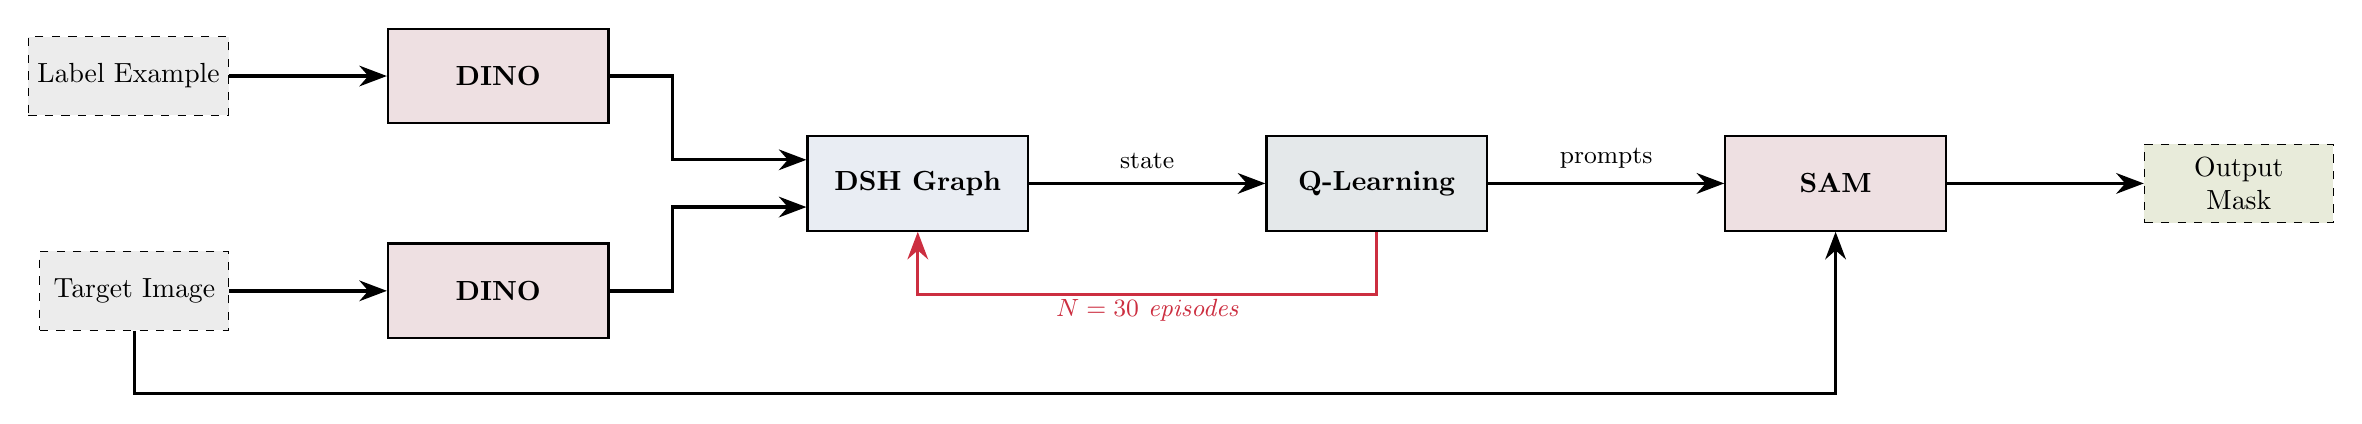
\begin{tikzpicture}[
    model/.style={
        draw, thick, minimum width=2.8cm, minimum height=1.2cm,
        align=center, font=\normalsize\bfseries
    },
    data/.style={
        draw, dashed, minimum width=2.4cm, minimum height=1.0cm,
        align=center, font=\normalsize
    },
    arr/.style={-{Stealth[length=3.5mm]}, very thick},
    lbl/.style={font=\small, fill=white, inner sep=2pt},
    every node/.style={font=\normalsize}
]

% =============================================
% TOP ROW: Label Example -> DINO
% =============================================
\node[data, fill=LightGray] (labelled) {Label Example};
\node[model, fill=Garnet!12, right=2.0cm of labelled] (dino1) {DINO};

% BOTTOM ROW: Target Image -> DINO (aligned exactly below)
\node[model, fill=Garnet!12, below=1.5cm of dino1] (dino2) {DINO};
\node[data, fill=LightGray, left=2.0cm of dino2] (target) {Target Image};

\draw[arr] (labelled.east) -- (dino1.west);
\draw[arr] (target.east) -- (dino2.west);

% =============================================
% CENTER: Graph, then Q-Learning to its right
% =============================================
\node[model, fill=Atlantic!12, right=2.5cm of $(dino1.east)!0.5!(dino2.east)$] (graph) {DSH Graph};

\draw[arr] (dino1.east) -- ++(0.8,0) |- ([yshift=0.3cm]graph.west);
\draw[arr] (dino2.east) -- ++(0.8,0) |- ([yshift=-0.3cm]graph.west);

\node[model, fill=Congaree!12, right=3.0cm of graph] (qlearn) {Q-Learning};

% Graph -> Q-Learning (top arrow)
\draw[arr] (graph.east) -- (qlearn.west)
    node[lbl, midway, above=0.1cm] {state};

% Q-Learning -> Graph update loop (bottom)
\draw[arr, Rose] (qlearn.south) -- ++(0,-0.8) -| (graph.south);
\node[font=\small\itshape, text=Rose] at ([yshift=-1.0cm]$(graph.south)!0.5!(qlearn.south)$) {$N = 30$ episodes};

% =============================================
% RIGHT: SAM and output
% =============================================
\node[model, fill=Garnet!12, right=3.0cm of qlearn] (sam) {SAM};

\draw[arr] (qlearn.east) -- (sam.west)
    node[lbl, midway, above=0.1cm] {prompts};

% Target image to SAM (arc underneath)
\draw[arr] (target.south) -- ++(0,-0.8) -| (sam.south);

\node[data, fill=Horseshoe!15, right=2.5cm of sam] (mask) {Output\\Mask};

\draw[arr] (sam.east) -- (mask.west);

\end{tikzpicture}
\end{document}
